\subsection{Spent Nuclear Fuel Simulations}
\label{sec:snfsim}

Because creating databases from real measurements to represent reactor
technologies from around the world is impossible, the database in this study
will be created from high-fidelity simulations via \gls{ORIGEN} \cite{origen},
a code used for activation, depletion, and decay of nuclear materials. It is a
part of the \gls{SCALE} 6.2 modeling and simulation suite of computational
tools developed for nuclear design and safety \cite{scale}. Specifically, the
ARP module of the ORIGEN code was used: \gls{ORIGEN-ARP}.

A set of simulations of \gls{SNF} at different burnups and cooling times will
comprise the database.  Of interest to an entity trying to create a weapon is
partially irradiated fuel if they have plutonium separations capabilities or
any radioactive substance in the case of a dirty bomb.  Addressing the former,
a smaller burnup than is typical for \gls{SNF} from a commercial reactor is
used in the previous work. This will be repeated here for demonstrative
purposes, but expanded upon in future work.

\begin{table}[!hp]
  \centering
  \begin{subtable}{\linewidth}
    \centering
    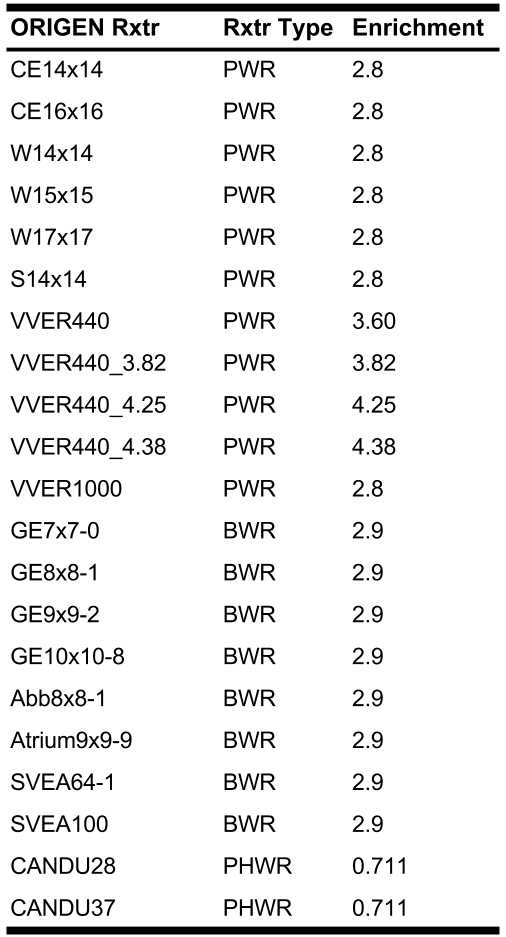
\includegraphics[height=0.7\textheight]{./chapters/demo_method/TrainData.png}
    \caption{Reactor types and uranium-235 enrichment [weight\%]}
    \label{tbl:rxtrtype}
    \vspace*{5mm}
  \end{subtable}
  \begin{subtable}{\linewidth}
    \centering
    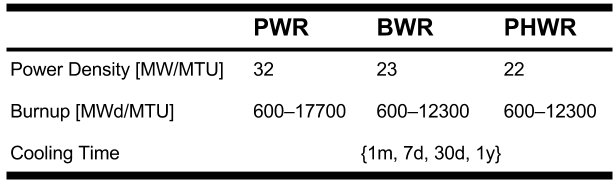
\includegraphics[width=0.7\linewidth]{./chapters/demo_method/TrainData2.png}
    \caption{Simulation space defining reactor parameters and cooling time}
    \label{tbl:rxtrparam}
  \end{subtable}%
  \caption{Design of the training set space}
  \label{tbl:train}
\end{table}

As mentioned in Section \ref{sec:optvalid}, many algorithms are developed on
the assumption that the training set will be \gls{i.i.d.}. This is important so
that the model does not overvalue or overfit a certain area in the training
space. As this is not easily proven, it requires extensive knowledge of
worldwide commercial reactors. Most obviously, a truly \gls{i.i.d.} training
set would go beyond the lower burnups, but this is purely for demonstration
with a single use case in mind.  The training database is thus constructed by
simulating the same training set space as described in Ref.
\cite{dayman_feasibility_2013}, shown in Table \ref{tbl:train}. For each entry
shown here the simulations included the span of cooling times and burnups in
\ref{tbl:rxtrparam}. 

\begin{table}[!hp]
  \centering
  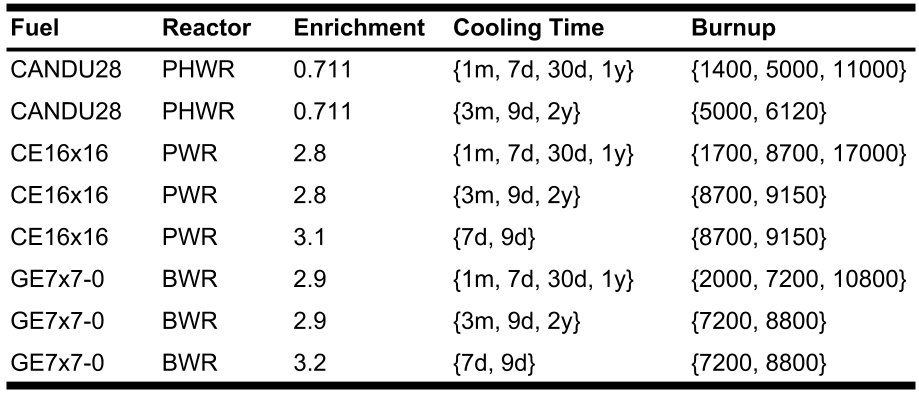
\includegraphics[width=0.95\linewidth]{./chapters/demo_method/TestData.png}
  \caption{Design of the testing set space}
  \label{tbl:test}
\end{table}

While in typical machine learning studies choose the testing set randomly from
the training set, the previous work used an external one, shown in Table
\ref{tbl:test}.  The test set was designed to have values in between the
trained values of burnup and cooling times for the same set of reactors.
However, a systematically chosen test set can be problematic since it may not
cover parts of the training space.  Therefore it was implemented in this study
for comparison, but cross-validation will be used moving forward. More
specifically, using \textit{k}-fold cross-validation is expected to better
indicate the model performance. 

\subsection{Information Reduction}
\label{sec:inforeduc}

Since the overall goal of this project is to determine how much information to
what quality is needed to train a machine-learned model, there will be an
information reduction manipulation applied to the training data set. This study
evaluates the impact of randomly introduced error on the ability of the
algorithms to correctly predict the burnup. 

The three algorithms will be evaluated with error applied to each nuclide
vector in the training set.  A maximum error ranging from $0 - 10\%$ is chosen
for each round of training, and a random error within the range of $[1-E_{max},
1+E_{max}]$ is applied to each component of the nuclide vector.

However, error in a nuclide vector is not random, in fact it is systematic and
dependent on a number of known sources of uncertainty. The next study will
introduce error by limiting the nuclides to only those that can be measured
with a gamma spectrometer. Although this is initially done using the
availability of gamma energies in \gls{ORIGEN}, \gls{GADRAS} can provide more
\gls{DRF}s to further reduce information given to the algorithm.

